\documentclass[12pt,a4paper]{article}

% Common preamble I use
\usepackage[utf8]{inputenc}         % Input encoding
\usepackage[T1]{fontenc}            % Font encoding
\usepackage{textcomp}               % Provides various additional symbols and text-related features
\usepackage{microtype}              % Improves micro-typography of the document
\usepackage{pifont}                 % Provides additional symbols, including dingbats
\usepackage{changepage}             % Allows adjustment of page layout parameters
\usepackage{ftnxtra}                % Allows for fancy footnotes
\usepackage{fancyhdr}               % Allows for headers and footers
\setlength{\headheight}{14.49998pt}
\addtolength{\topmargin}{-2.49998pt}
\usepackage{subcaption}             % Enhanced support for sub-figures and sub-captions
\usepackage{wrapfig}

\usepackage{chemgreek,textgreek}    % Greek letters 

\usepackage{authblk}                % For customizing author block layout in the title page

% Listings setup
\usepackage{listings}               % Code listings
\usepackage{xcolor}                 % Color support
% Define R language for listings
\lstdefinelanguage{R}{
    keywords={function,
              if,
              else,
              repeat,
              while,
              for,
              in,
              next,
              break,
              TRUE,
              FALSE,
              NULL,
              Inf,
              NaN,
              NA,
              NA_integer_,
              NA_real_,
              NA_complex_,
              NA_character_,
              library,
              require,
              install.packages},
    keywordstyle=\color{blue}\bfseries,
    sensitive=true,
    comment=[l]{\#},
    commentstyle=\color{green!50!black},
    stringstyle=\color{orange},
    morestring=[b]'',
    morestring=[b]',
    moredelim=[is][\color{purple}]{`}{`}
}
\lstdefinestyle{Rstyle}{
    language=R,                
    basicstyle=\ttfamily\small,
    keywordstyle=\color{blue}, 
    stringstyle=\color{orange},
    commentstyle=\color{green!50!black}, 
    backgroundcolor=\color{gray!10},    
    showstringspaces=false,    
    numbers=left,              
    numberstyle=\tiny,         
    breaklines=true,           
    frame=single,              
}

% Graphic packages
\usepackage{graphicx}               % Graphics support
\usepackage[a4paper, margin=1in]{geometry}
\usepackage{tikz}                   % For in-doc drawings
\usepackage{pgfplots}
\pgfplotsset{compat=1.18}

% Maths packages
\usepackage{amsmath}                % Math support
\usepackage{amssymb}                % Provides various additional mathematical symbols
\usepackage{amsthm}                 % Provides enhanced support for theorem-like environments

% Table support packages
\usepackage{xtab}                   % Tables with adjustable width 
\usepackage{multirow}               % For multi-row cells in tables
\usepackage{array}                  % Provides more flexible and customizable array and tabular environments
\usepackage{longtable}              % Allows tables that span multiple pages
\usepackage{threeparttablex}        % Helps avoid clashes between tables and footnotes
\usepackage{tabularray}             % Combines features of longtable, array, multirow, etc.

\usepackage{booktabs}               % Enhanced tables
\usepackage{csquotes}               % Quotation marks and quote formatting
\usepackage{siunitx}                % For typesetting numbers and units.
\sisetup{                           % Centers numbers in tables by the decimal point.
  input-ignore={,},
  input-decimal-markers={.},
  group-separator={,},
  table-align-text-pre=false,
  table-align-text-post=true
  }

\usepackage{algorithm}              % Allows insertion of algorithms as an object
\usepackage{algpseudocode}          % Used to insert pseudocode  
\usepackage{caption}                % Customizes captions in floating environments

\usepackage{setspace}

\usepackage{ragged2e}               % Enhanced text alignment commands

\usepackage{enumitem}               % Customizable lists     

\usepackage[sort&compress]{natbib}  % Cite style
\setcitestyle{numbers,square,comma}

\usepackage{times}                  % Times font       

\usepackage{hyperref}               % Hyperlinks
\usepackage{url}                    % For typesetting URLs with line breaks at hyphens
\def\UrlBreaks{\do\/\do-}           % Allows urls to break lines chktex 4
\hypersetup{breaklinks=true}
\urlstyle{same}
\usepackage{nameref}                % Enables referencing section names instead of numbers

% For using TODO notes
% \todo[inline,caption={}]{TODOs are to be inserted like this}
%\usepackage[color=blue!10,textsize=footnotesize,textwidth=25mm]{todonotes}
%\usepackage[disable]{todonotes}
\usepackage{float}

% CUSTOM LABELS
\DeclareCaptionLabelFormat{apafigure}{\textbf{Figure #2}}
\DeclareCaptionLabelFormat{procedure}{\textbf{Procedure #2}}
\DeclareCaptionLabelFormat{apalisting}{\textbf{Listing #2}}

% CUSTOM CAPTION FORMATS
\captionsetup[figure]{labelformat=apafigure,
                      labelsep=newline,
                      justification=justified,
                      singlelinecheck=false}
\DeclareMathOperator{\atan}{atan}
\captionsetup[lstlisting]{labelformat=apalisting,
                          position=above,
                          justification=raggedright,
                          labelsep=newline,
                          singlelinecheck=false,}
\DeclareCaptionLabelSeparator*{spaced}{\\[2ex]}
\captionsetup[table]{textfont=bf,
                     format=plain,
                     justification=justified,
                     singlelinecheck=false,
                     labelsep=newline,
                     skip=0pt}

\makeatletter
% Commands to format a counter value as Greek letter to be used like 
% \arabic or \roman when using enumerate:
\newcommand*\alphgreek[1]{\expandafter\@alphgreek\csname c@#1\endcsname}
\newcommand*\@alphgreek[1]{\csname chemgreekIntToGreek:n\endcsname{#1}}
\newcommand*\Alphgreek[1]{\expandafter\@Alphgreek\csname c@#1\endcsname}
\newcommand*\@Alphgreek[1]{\csname chemgreekIntToGreek:n\endcsname{#1}}

% Register new counter formats to enumitem:
\AddEnumerateCounter*{\alphgreek}{\@alphgreek}{\chemalpha}
\AddEnumerateCounter*{\Alphgreek}{\@Alphgreek}{\chemAlpha}
\makeatother

% \code{} command to insert in-text code snippets
\definecolor{light-gray}{gray}{0.95}
\newcommand{\code}[1]{\colorbox{light-gray}{\texttt{#1}}}

% AUTHOR
\newcommand{\authorname}{Samuel Jonsson}
\newcommand{\authormail}{\href{mailto:sajs19@student.bth.se}{sajs19@student.bth.se}}
\newcommand{\authorpersonnr}{19990415-5596} % chktex 8
\newcommand{\program}{DVAMI19h}

% REPORT METADATA
\newcommand{\doctitle}{MS2505: Bayesian Statistics}
\newcommand{\docsubtitle}{Course Project}
\newcommand{\docdate}{Latest version: \today}

\pagestyle{fancy}                                 % Use the fancy page style
\fancyhf{}                                        % Clear all headers and footers

% HEADER CUSTOMISATION
\fancyhead[L]{\textit{\doctitle~--~\docsubtitle}} % Header float left
\fancyhead[R]{\textit{\docdate}}                  % Header float right

% FOOTER CUSTOMISATION
\fancyfoot[L]{\authorname~--~\authormail}         % Footer float left
\fancyfoot[R]{Page \thepage}                      % Footer float right

\setlist{topsep=1ex,itemsep=0.5ex,parsep=0pt,partopsep=0pt}

\begin{document}

\vspace*{3cm}

\begin{center}
    \Huge\textbf{\doctitle}\\
    \Large\textbf{\docsubtitle}
    \\\vspace*{5mm} 
    \large\today                            
\end{center} 

\vspace*{1cm}
\begin{center}
    \textit{Name}       \\
    \authorname         \\ % chktex 1
    \vspace*{2mm}
    \textit{Email}      \\
    \authormail         \\ % chktex 1
    \vspace*{2mm}
    \textit{Person Nr.} \\
    \authorpersonnr     \\ % chktex 1
    \vspace*{2mm}
    \textit{Program}    \\
    \program               % chktex 1
\end{center}

\begin{figure}[!b]
    \centering
    
\includegraphics[width = 0.25\textwidth]{../figures/BTH_logo_black.png}
\end{figure}

\newpage

\section{Analysis problem}\label{sec:analysisproblem}

The analysis aims to estimate the proportion of emails classified as spam in a given dataset. Using Bayesian
methods, the focus is on deriving a reliable estimate of this proportion while accounting for uncertainty.
The simplicity of the approach allows for clear insights into the spam classification problem, although it
abstracts away complexities like email content or contextual nuances. The objective is to provide a robust
probabilistic framework for understanding the distribution of spam within the dataset.

\section{Data Description}\label{sec:datasdescription}
The dataset selected for this project was obtained from
\href{https://www.kaggle.com/datasets/venky73/spam-mails-dataset}{Kaggle} and consists of labeled email
messages, where each email is classified as either ``spam'' or ``ham''. The dataset contains the following
columns:
\begin{itemize}
    \item \textbf{Category}: A binary label indicating whether the email is spam ($1$) or ham ($0$).
    \item \textbf{Message}: The text content of the email.
\end{itemize}
The first 10 rows of the dataset are shown in Table~\ref{tab:maildata}. For this analysis, the focus is on
the Category column, which serves as the response variable for the Bayesian classification model.

\setcounter{table}{0}

\begin{longtable}[!ht]{p{2cm}|p{11cm}}
    \caption{\code{mail\_data.csv} dataset first 10 rows}                                               \\
    \label{tab:maildata} % chktex 24
    \textbf{Category} & \textbf{Message}                                                                \\
    \hline % chktex 44
    ham      & ``Go until jurong point, crazy.. Available only in bugis n great world la e buffet\dots
               Cine there got amore wat\dots''                                                          \\
    \hline % chktex 44
    ham      & Ok lar\dots Joking wif u oni\dots                                                        \\
    \hline % chktex 44
    spam     & Free entry in 2 a wkly comp to win FA Cup final tkts 21st May 2005. Text FA to 87121 to
               receive entry question (std txt rate) T\&C's apply 08452810075over18's                   \\
    \hline % chktex 44
    ham      & U dun say so early ho\dots U c already then say\dots                                     \\
    \hline % chktex 44
    ham      & ``Nah I don't think he goes to usf, he lives around here though''                        \\
    \hline % chktex 44
    spam     & ``FreeMsg Hey there darling it's been 3 week's now and no word back! I'd like some fun you
                up for it still? Tb ok! XxX std chgs to send, \pounds1.50 to rcv''                      \\
    \hline % chktex 44
    ham      & Even my brother is not like to speak with me. They treat me like aids patent.            \\
    \hline % chktex 44
    ham      & As per your request ´Melle Melle (Oru Minnaminunginte Nurungu Vettam)' has
               been set as your callertune for all Callers. Press *9 to copy your friends Callertune    \\
    \hline % chktex 44
    \dots    & \dots                                                                                    \\
\end{longtable}

Using a python script, the labels are then converted to numerical values, where spam is represented as $1$
and ham as $0$. After preprocessing the data, the dataset contains a total of 
\begin{longtable}[!ht]{p{3cm}p{10cm}}
    747  & Spam         \\
    4825 & Ham          \\
    5572 & Total Emails \\
\end{longtable}

\setcounter{table}{1}

These counts are used to update the beta distribution's prior parameters and compute the posterior
distribution.

Then, using a Python script, the labels were converted to $1$ if it was ``spam'' and $0$ if it was ``ham'',
for easier analysis.

\section{Model}\label{sec:model}
The model chosen for this analysis is a binomial likelihood model with a beta prior. This approach is
particularly suitable for binary classification problems where the response variable is dichotomous,
such as classifying emails as either ``spam'' ($1$) or ``ham'' ($0$).

The binomial likelihood model represents the probability of observing a given number of successes (spam)
in a fixed number of trials (emails). The parameter of interest, $\theta$, represents the probability of
an email being classified as spam. Using this model allows us to estimate $\theta$ while accounting for
uncertainty.

To complement the likelihood, we use a $Beta(1,1)$ prior, which is non-informative and reflects a state of
prior ignorance about $\theta$. This choice aligns with common practices in Bayesian analysis, particularly
when no strong prior knowledge exists. By combining the prior with the observed data, we compute the
posterior distribution of $\theta$, providing a probabilistic estimate of the spam probability.

In addition, Markov Chain Monte Carlo (MCMC) methods are employed to validate the results obtained from the
closed-form posterior distribution. MCMC sampling allows us to approximate the posterior distribution of 
$\theta$ when the analytic computation becomes infeasible.

\section{Results}\label{sec:results}

This section presents the outcomes of the Bayesian analysis performed using a Beta-binomial model to estimate
the probability ($\theta$) that an email is classified as spam. Results from Monte Carlo and MCMC sampling
methods are summarized and validated, followed by visualizations to illustrate the posterior distributions
and sampling behavior.

\subsection{Posterior Analysis}\label{ssec:posterioranalysis}

Monte Carlo sampling, performed with 10,000 draws from the posterior distribution of $\theta$, provides a
detailed summary of the key statistics in Table~\ref{tab:posterioranalysistable}. The posterior mean estimate
for  $\theta$ is approximately 13.42\%, with a narrow 95\% credible interval of $[0.125,0.143]$. This
suggests a high degree of confidence in the estimate and indicates that, on average, 13.42\% of emails are
classified as spam.

\begin{longtable}[!ht]{p{4cm}|p{11cm}}
    \caption{Monte Carlo Posterior Analysis Data}   \\
    \label{tab:posterioranalysistable}  % chktex 24
    \textbf{Posterior Mean} & $0.1341994$           \\
    \hline                              % chktex 44
    \textbf{Posterior SD} & $0.004576791$           \\
    \hline                              % chktex 44
    \textbf{95\% Credible Interval} & $[0.1252803, 0.1432051]$
\end{longtable}

\subsection{MCMC Validation}\label{ssec:mcmcvalidation}

To validate the results, MCMC sampling was performed using the \code{MCMCmetrop1R} function. As shown in
Table~\ref{tab:mcmcposterioranalysistable}, the posterior mean is consistent at 13.44\%, with a 95\%
credible interval of $[0.125,0.144]$. These results further confirm the robustness of the estimates and
align closely with the Monte Carlo findings.

\begin{longtable}[!ht]{p{4cm}|p{11cm}}
    \caption{MCMC Posterior Analysis Data}  \\
    \label{tab:mcmcposterioranalysistable}  % chktex 24
    \textbf{Posterior Mean} & $0.1344085$   \\
    \hline                                  % chktex 44
    \textbf{Posterior SD} & $0.004670508$   \\
    \hline                                  % chktex 44
    \textbf{95\% Credible Interval} & $[0.1254781, 0.1437142]$ 
\end{longtable}

The strong agreement between the Monte Carlo and MCMC methods demonstrates the model's validity and the
consistency of the Bayesian inference process.

\subsection{Visualization}\label{ssec:visualisations}

The posterior distributions derived from Monte Carlo and MCMC sampling are visualized in
Figures~\ref{fig:posterior} and~\ref{fig:mcmcposterior}, respectively. Both distributions exhibit a sharp
peak around $\theta \approx 0.135$, reflecting the central tendency of the estimates.

\begin{figure}[!ht]
    \centering
    \begin{subfigure}{0.49\textwidth}
        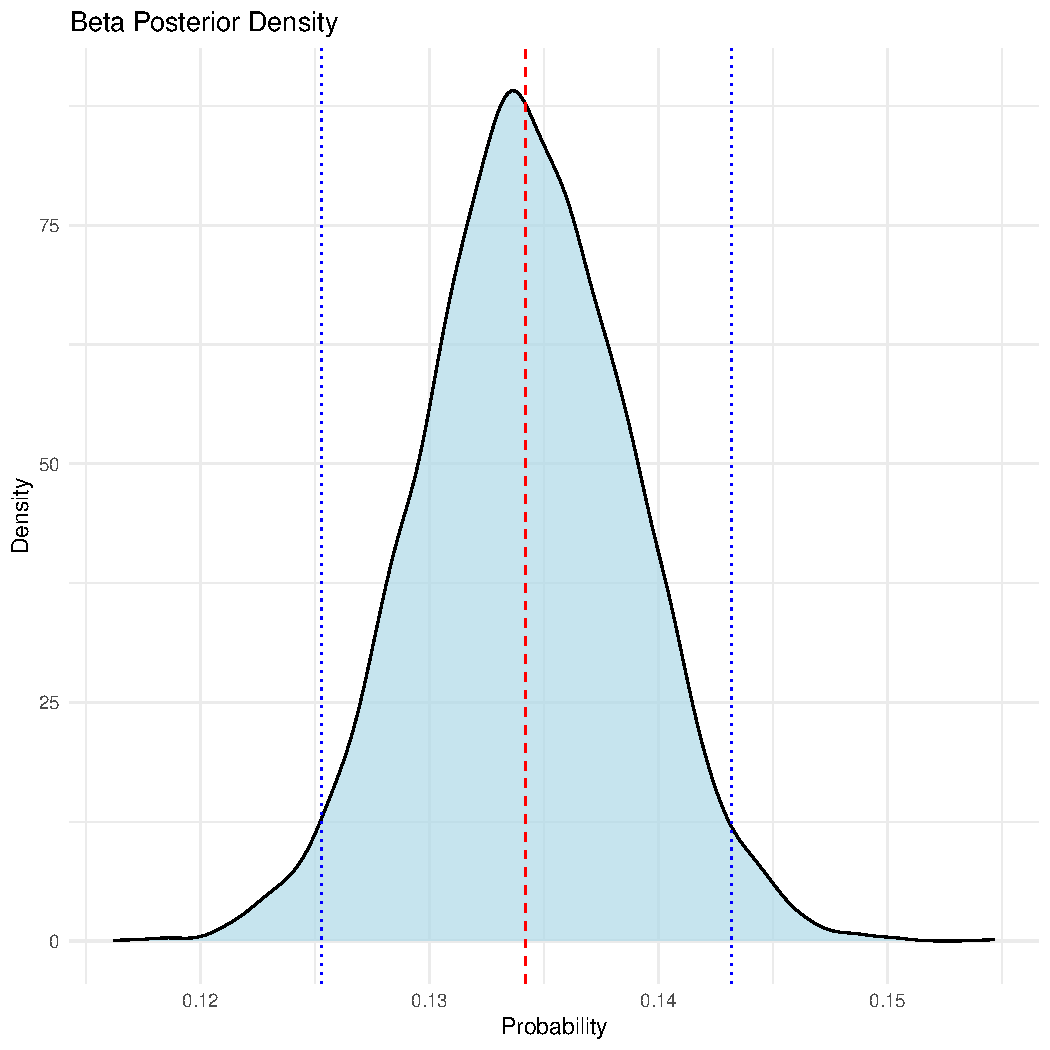
\includegraphics[width=\textwidth]{figures/beta_posterior_density_plot.pdf}
        \caption{Density plot}\label{fig:posteriordensityplot}
    \end{subfigure}
    \begin{subfigure}{0.49\textwidth}
        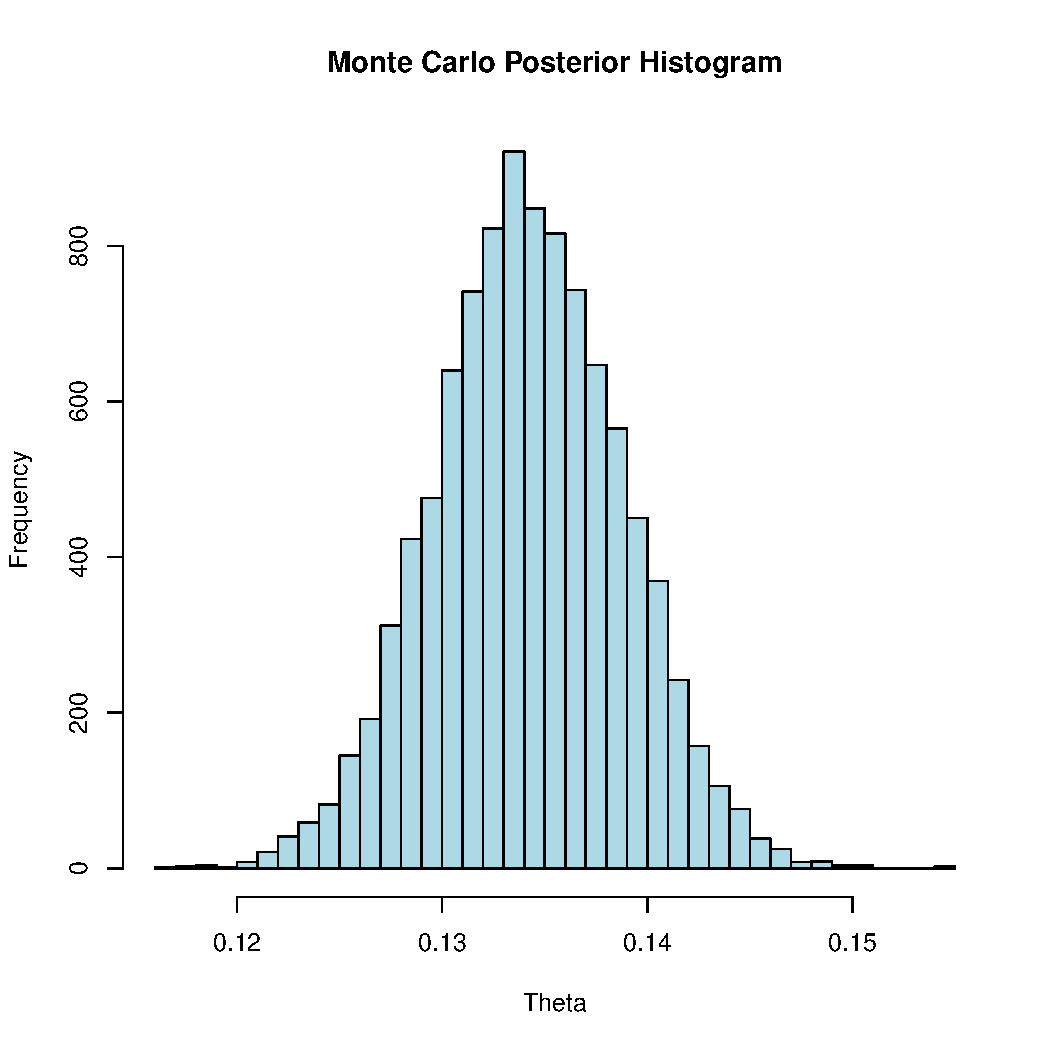
\includegraphics[width=\textwidth]{figures/beta_posterior_histogram.pdf}
        \caption{Histogram}\label{fig:posteriorhistogram}
    \end{subfigure}
    \caption{Posterior density and histogram for Monte Carlo sampling. The sharp peak
    at $\theta \approx 0.135$ aligns with Table~\ref{tab:posterioranalysistable}.}\label{fig:posterior}
\end{figure}

Similarly, the MCMC posterior density and histogram (Figure~\ref{fig:mcmcposterior}) reveal consistent
results, reinforcing the robustness of the Bayesian model.

\newpage

\begin{figure}[!ht]
    \centering
    \begin{subfigure}{0.49\textwidth}
        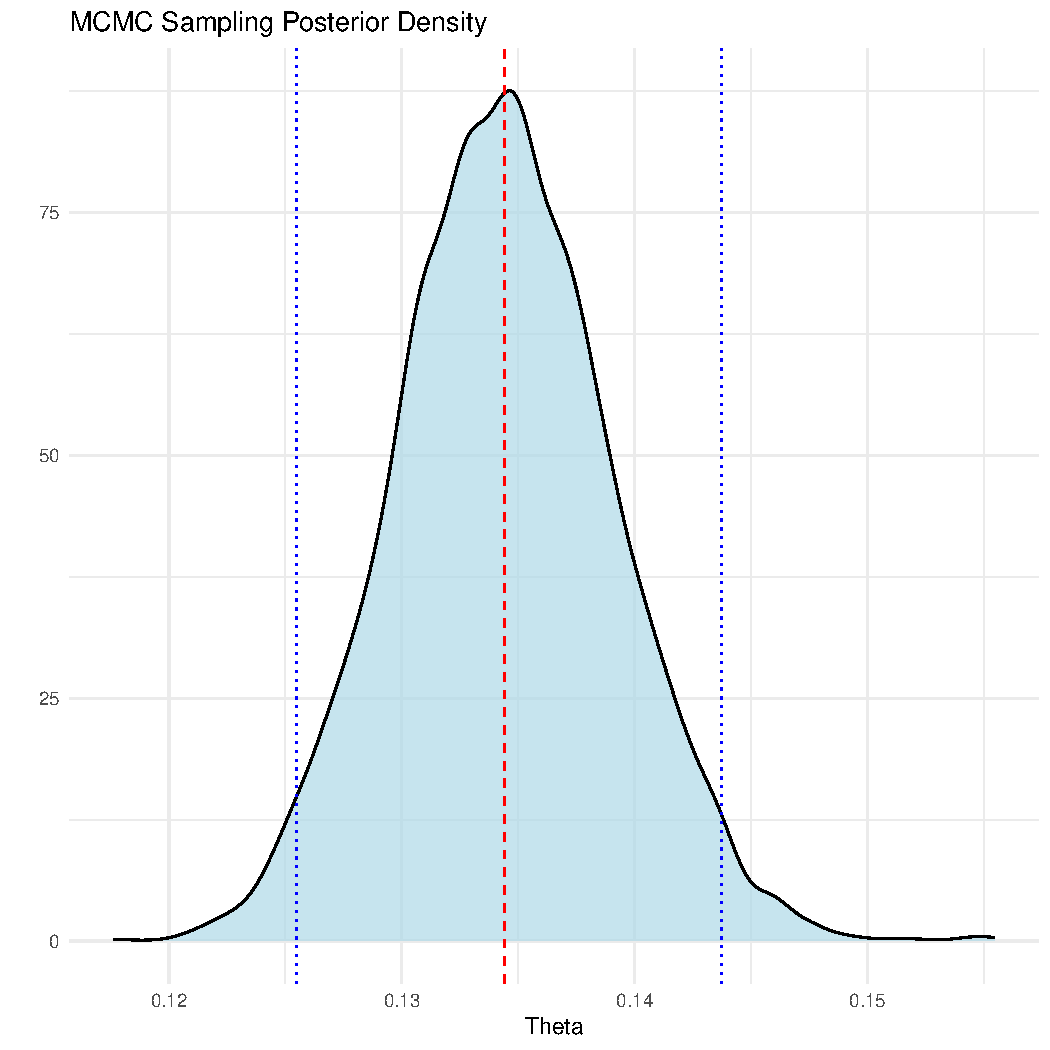
\includegraphics[width=\textwidth]{figures/mcmc_posterior_density_plot.pdf}
        \caption{MCMC density plot}\label{fig:mcmcposteriordensityplot}
    \end{subfigure}
    \begin{subfigure}{0.49\textwidth}
        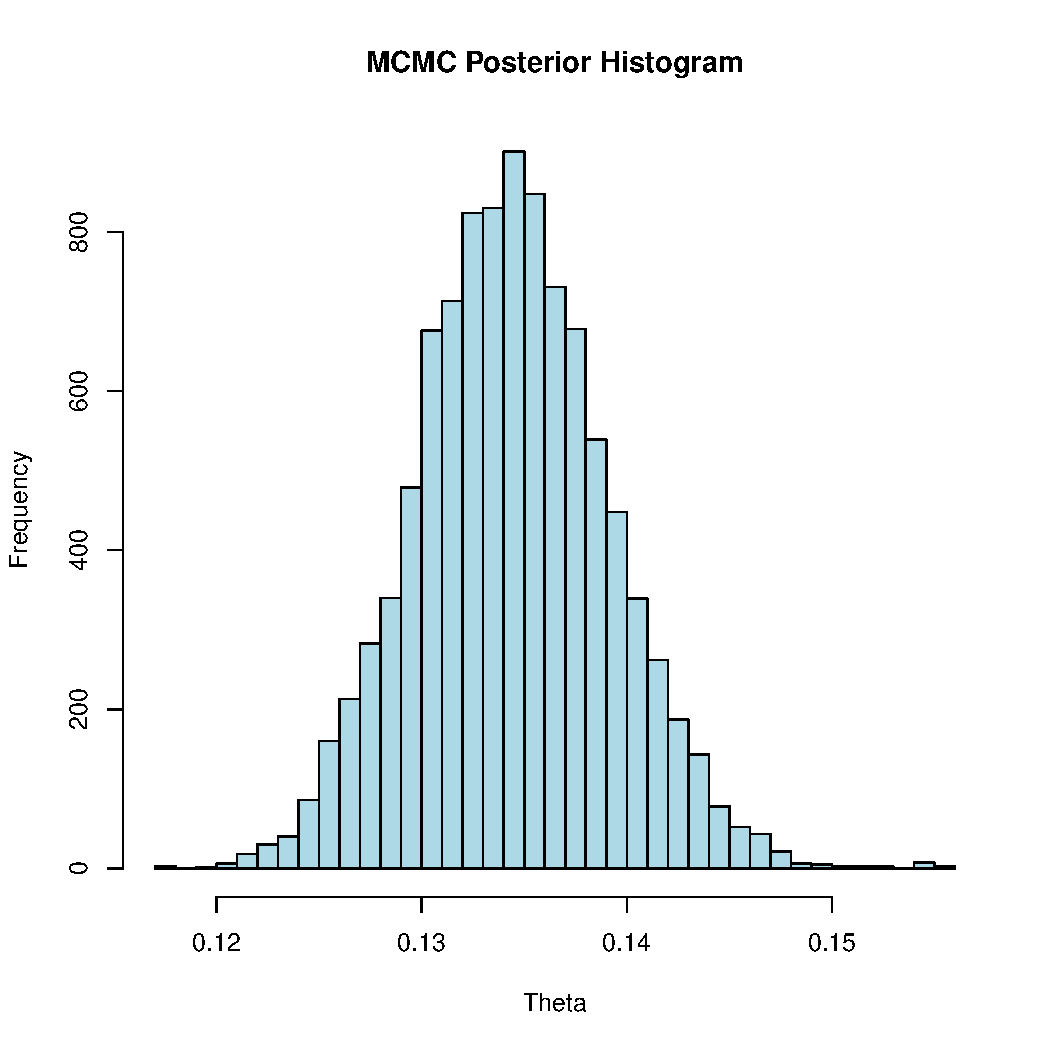
\includegraphics[width=\textwidth]{figures/mcmc_posterior_histogram.pdf}
        \caption{MCMC histogram}\label{fig:mcmcposteriorhistogram}
    \end{subfigure}
    \caption{Posterior density and histogram for MCMC sampling, demonstrating consistency with Monte Carlo
    results and Table~\ref{tab:mcmcposterioranalysistable}.}\label{fig:mcmcposterior}
\end{figure}

The tails of the posterior distributions provide additional insights into the uncertainty associated with
$\theta$. Both Monte Carlo and MCMC density plots show symmetric tails that taper quickly beyond the 95\%
credible intervals, indicating a low likelihood of extreme values. Sparse population in the outer bins of
the histograms further highlights the concentration of posterior mass near the central estimates. Slightly
broader tails in the MCMC density plot compared to the Monte Carlo results may suggest minor differences in
sampling variability, though these are negligible in the overall context of the model's consistency and
reliability.

\subsection{MCMC Trace Plot}\label{ssec:traceplot}

The trace plot of the MCMC samples (Figure~\ref{fig:mcmctraceplot}) provides further evidence of the sampling
process's stability and convergence. The sampled values oscillate consistently around a central range without
noticeable trends or significant deviations, confirming that the chain has reached a stationary distribution.

\newpage

\begin{figure}[!ht]
    \centering
    \begin{minipage}[ht]{0.6\textwidth}
        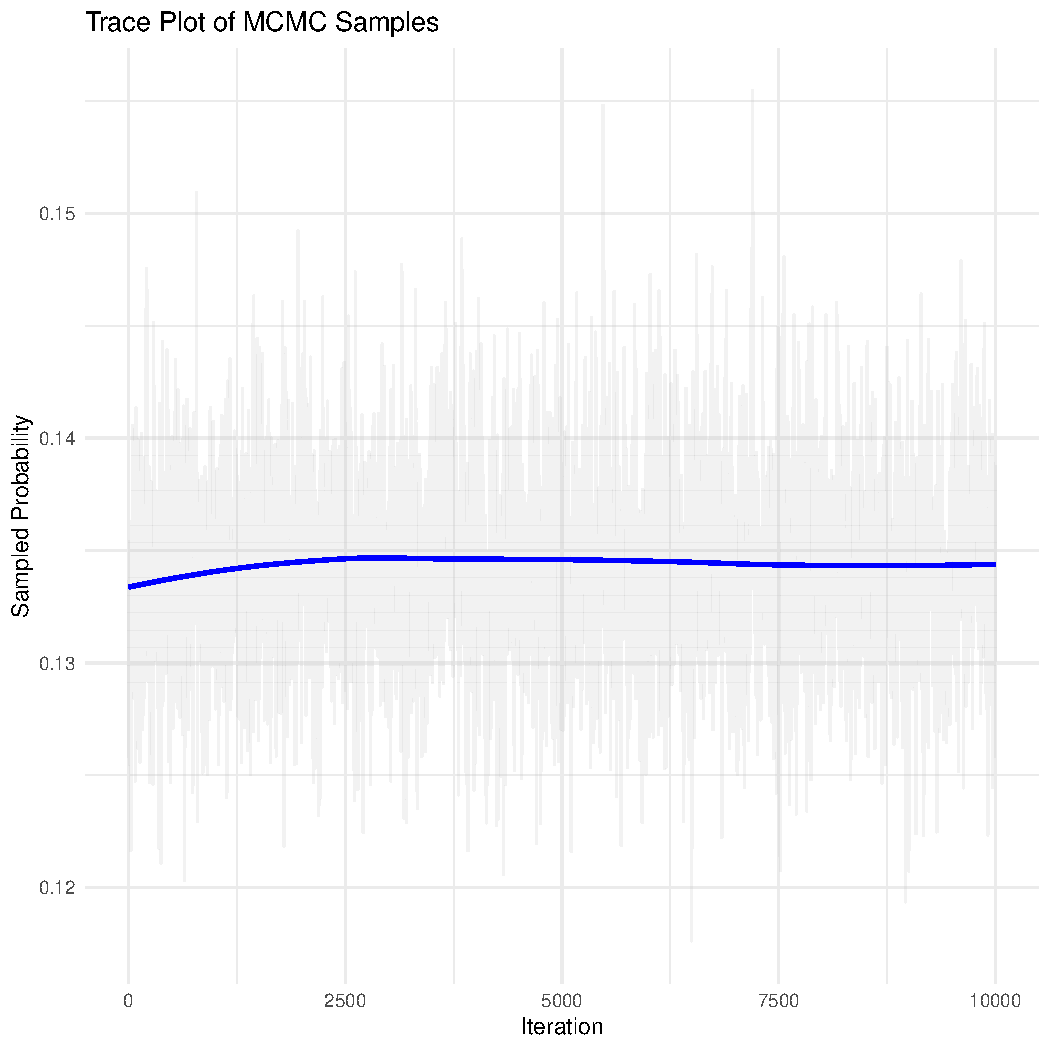
\includegraphics[width=\textwidth]{figures/mcmc_trace_plot.pdf}
    \end{minipage}
    \hspace{0.02\textwidth}
    \begin{minipage}[ht]{0.35\textwidth}
        \caption{MCMC sampling trace plot. The stable fluctuations confirm convergence to the posterior distribution.}
        \label{fig:mcmctraceplot} % chktex 24
    \end{minipage}
\end{figure}

This stable behavior, along with minimal autocorrelation and effective mixing, suggests that the MCMC samples
are representative of the posterior distribution. While minor clustering is observed in certain regions of
the plot, this does not significantly affect the validity of the estimates.

\section{Discussion}\label{sec:discussion}

The Bayesian analysis conducted in this project produced reliable and consistent results for estimating the
probability $\theta$ that an email is classified as spam. As mentioned in Section~\ref{sec:model}, the
simplicity of the Beta-binomial model provided a clear and computationally efficient approach for this
foundational analysis. Both Monte Carlo and MCMC sampling methods yielded posterior mean estimates of
approximately 13.4\%, with narrow 95\% credible intervals, demonstrating a high level of confidence in the
central estimate. The visualizations, discussed in Section~\ref{ssec:visualisations}, further supported these
findings, revealing well-behaved posterior distributions with symmetric tails and rapid tapering, reflecting
low uncertainty around the estimates. Additionally, the trace plot in Section~\ref{ssec:traceplot} confirmed
convergence of the MCMC sampling process, with sampled values stabilizing without significant deviations.

However, while the Beta-binomial model provides a straightforward and computationally efficient framework,
it has inherent limitations. As mentioned in Section~\ref{sec:model}, the model focuses on binary
classification, treating emails as either spam ($1$) or ham ($0$). This simplicity, while beneficial
for interpretability, abstracts away complexities such as email content or metadata, which could provide
richer insights into spam classification. Consequently, this approach restricts the model's ability to
generalize to unseen datasets with varying characteristics. Additionally, the choice of a $Beta(1,1)$ prior
assumes no prior knowledge about the data, which, while this neutral stance aligns with the exploratory
nature of the analysis, it may not optimally reflect datasets with unusual or heavily skewed properties.

To address these challenges, several improvements could be explored. First, as noted in
Section~\ref{sec:datasdescription}, the dataset contains the email text content, and incorporating this
into the model could enhance its predictive capabilities, allowing it to better generalize to diverse or
unknown datasets. For instance, incorporating natural language processing techniques to analyze the textual
content could provide additional predictors beyond the binary classification framework. Additionally,
extending the model to include hierarchical structures, as a refinement of the foundational framework
described in Section~\ref{sec:model}, could capture variations across subpopulations or different
email sources, offering a more nuanced understanding of $\theta$.

The choice of prior distribution, discussed in Section~\ref{sec:model}, is another area for potential
improvement. Rather than using a neutral $Beta(1,1)$ prior, future analyses could explore data-informed
priors that align with specific dataset characteristics. For instance, if prior information about spam
prevalence is available from other sources, it could be incorporated to improve the robustness and
sensitivity of the posterior analysis. The nature of the problem, however, would making a generally
representative prior quite challenging, as the number of spam emails in an unknown dataset would be
difficult to determine without more contextual knowledge. 

On the computational side, the MCMC sampling methods, while effective, could benefit from the adoption
of advanced techniques such as Hamiltonian Monte Carlo or adaptive MCMC methods. As noted in
Section~\ref{ssec:mcmcvalidation}, MCMC sampling produced slightly broader tails compared to Monte Carlo
sampling, suggesting some variability in the results. Enhanced sampling techniques could reduce this
variability while improving computational efficiency.

In summary, while the simplicity of the beta-binomial model proved effective for this initial analysis, it
highlights a trade-off between clarity and flexibility. The straightforward approach ensured interpretable
results and computational feasibility. However, the challenges discussed here underscore the need for a more
comprehensive framework in future analyses. Building on the current findings, incorporating richer features,
hierarchical structures, and optimized priors would enhance the model's applicability to real-world spam
detection scenarios. This iterative refinement process is essential for balancing simplicity with the
complexities of dynamic and diverse datasets.

\newpage
\section{Appendix}
\appendix
\section{R Code}
\lstinputlisting[language=R,style=Rstyle,caption=Project R code,label=apx:RCode,]{./project.r}

\end{document}